\section{Analysis of \sse Output}\label{sec:ana}

Each execution of \sse creates a folder for analysis output.
Apart from the general log files, where all plugins write important messages, some plugins also create separate files.
For instance one file contains performance characteristics of the test run, another one LLVM bytecode of all analysed programs.
The exact numbers and types of output files depend on which plugins are defined in \sse's configuration Lua script.

The most important information about \sse's general execution is accumulated in \textit{messages.txt}.
Backbone of this file is information about all execution paths, at which memory addresses they were forked, how they are constrained, when and why they were terminated, and much more.
%But it is also used by other plugins...
It is also the place where we saved all custom log messages as defined in the previous chapter to.

\medskip

Thanks to the clear structure of \textit{messages.txt} it can be used as input for a custom Python script. This script was written in order to visualise the \textbf{tree of execution paths} graphically, which serves as a great help with understanding path forking behaviour.
Figure \ref{fig:tree} shows the vital part of the tree of execution paths of \app.

Each box represents an execution state, lines pointing to another state symbolise a fork of the execution state.
The hexadecimal number at the origin of each edge is the memory address in which the state was forked.
For the sake of clarity I also manually added the function in which each memory address occurs.

Edges are labelled with constraints that need to be respected in the corresponding execution state.
KLEE handles constraints in Extended Backus-Naur Form syntax (e.g., \textit{``(Not (Slt (w32 0x20a1) (ReadLSB w32 0x0 v0\_income\_0)))''} for $``income \ge 8353''$).
For simplicity all constraints were also manipulated manually and transformed into a more readable format.

%Blue state boxes indicate one connection to the internet so far, yellow two and red three.
The text below each leaf shows the output of the \textit{TestCaseGenerator} plugin for this execution path.
Upon termination of a state it finds concrete input examples for the two symbolic variables $income$ and $taxcat$.

\medskip

Before coming to the actual research objectives of this paper, namely finding privacy problems, a quick interpretation of the bare tree shown in figure \ref{fig:tree} helps to gain a common understanding of \app.

Program execution largely relies on two integer variables, $income$ and the tax category $taxcat$.
Most forks in the assembly function $main()$ seem to be basic checks if these two variables contain valid data (e.g., $[taxcat > 6]$).
This assumption arises from the fact that many of these forks are leaves which exist only a very short time and consume hardly any memory (can be checked via the \textit{MemoryChecker} plugin).
These paths are probably error cases that terminate the program.

Important logic seems to take place in a function called \textit{calc\_tax()}.
Many forks originate in this method and both symbolic variables play a role in it.
Important in this case means `important with respect to being relevant to the symbolic execution of the two focal variables $income$ and $taxcat$'.
Paths with the constraints $[income < 13468]$ and $[income < 52880]$ seem to be less important since they are leaves in the tree.
The two paths $[52880 \le income < 250729]$ and $[income \ge 250729]$, however, entail further checks of $taxcat$, the other symbolic variable.
Summarising the general findings so far, \app checks the user's income and tax category and takes special actions if the income is higher than 52880 euros.

Unfortunately, due to the problem with incomplete test results (described at the end of this chapter), the tree in figure \ref{fig:tree} does not show all execution states.
While many states (900+) were manually left out due to insignificance, many more states are missing in \sse's output despite potentially being relevant.
For example, we cannot say what happens if $income$ is below or equal 8353 (the complementary event of the switch from state 3 to state 4).

\begin{figure*}
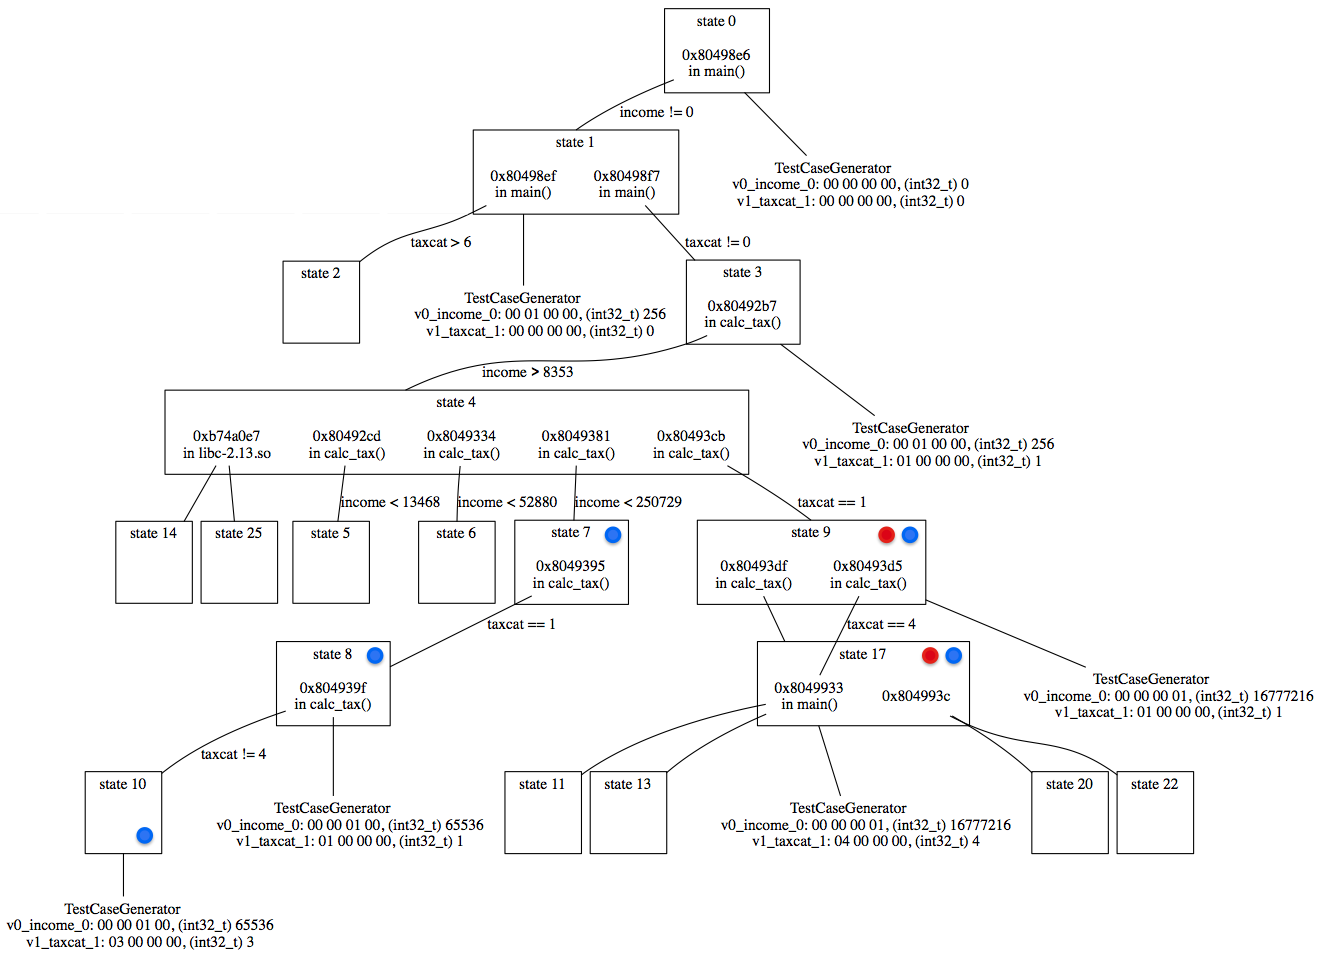
\includegraphics[width=\textwidth]{cool4}
\caption{Tree visualisation for understanding path forking behaviour in the analysis of \app. Shows at which memory addresses \sse forked new execution states. Path constraints are printed at each state transition. For most states, the \textit{TestCaseGenerator} found meaningful concrete example values for the two symbolic variables $income$ and $taxcat$. Blue dots symbolise that in this state a ``donation'' message was transferred to a server. Red dots mark states which leak the complete set of user inputs.}
\label{fig:tree}
\end{figure*}

\medskip

After this general inspection of \app's behaviour, we can finally shift the focus towards the research objectives regarding privacy issues.
As described in the previous chapter, \sse was programmed to monitor all instructions related to connections to the internet.
Output of these inspection activities have to be extracted from the \sse's main log file.
%Viewing those custom logs in the context of all other important \sse messages facilitates the interpretation of connections in the
Based on the output resulting from annotating the function \textit{send\_data}, which includes reading out the parameter the method is called with (see listing \ref{lst:send_data}), messages sent to the internet can be classified into three categories:
\begin{enumerate}
\item A command ``load\_ad'', which leads to a server response containing an advertisement for the user.
\item A command ``donate'', which entails a static message from the server prompting the user to donate to the poor programmer. \medskip \\
Output messages $1.)$ and $2.)$ do not contain any further data apart from the command.
\item A message depending on both symbolic variables $income$ and $taxcat$.
It always starts with the keyword ``found\_hit'', followed by all data the user has entered.
Message fields are separated by a colon and stick to the order `user name', `birth date', `income' and `tax category'. Example: ``found\_hit:name:1.1.77:16777216:1''.
Response from the server is a static status message.
\end{enumerate}

While message type $1.)$ could be expected (\app informed us that it shows advertisements), calls for donation (type $2.)$) were not announced before.
Still, since ``donate'' messages here do not contain any user-specific data, at this point of the analysis they can be considered innocuous with regard to privacy issues.

Internet connections of type $3.)$, however, undoubtedly impair the user's privacy.
They send the whole set of confidential user data to a server in the internet.
Hence a clear answer to research question three is: yes, \app does leak personal data of the user!

Note that even if \app would try to disguise its actions by encrypting the data it sends to the server, \sse would still find out which symbolic variables the encrypted message depends on.
Thus it should be possible to find out what data is sent even without thorough analysis of the encryption mechanisms.

\medskip

Now that all different connections to the internet are unveiled, we want to take advantage of \sse's ability to pursue all possible execution paths and find out in which cases \app connects to the internet.

For this purpose the execution tree in figure \ref{fig:tree} was enriched with the information in which execution state which connections to the internet took place.

Blue dots in the graph mark that this state triggered a donation call (message of type $2.)$).
A look at path constraints in these states tells that the common criteria here must be an $income$ either between 52880 and 250729 or even above 250729 euros.
Apparently the programmer assumed wealthy people to be more generous than those with a low income.
Despite the fact that these type $2.)$ calls do not transfer any user data to the server, they may potentially be a delicate matter since merely triggering them implicitly reveals information about the current user's income to the server.

Red dots in the tree visualise a message leaking data in this state (message type $3.)$).
Since all affected states originate at the fork in memory address $0x80493cb$, one condition for type $3.)$ connections must be an $income$ above 250729 euros.
Results of the \textit{TestCaseGenerator} plugin for the states 9 an 17 confirm this observation.
Additionally, path constraints require $taxcat$ to be either 1 or 4 in order to trigger this type of connection.
Obviously the evil programmer of \app is only interested in data of users with a very high income and tax category one or four.

The advertisement was loaded in every state, so this connection was not marked in the execution tree.
\app's source code apparently triggers the call for an advertisement before checking anything related to the symbolic variables $income$ and $taxcat$.



Since \sse eventually finds all possible execution paths of a program (if configured to do so), we can be sure that we did not miss any message type or occasion where connections are established.
When simply debugging \app it is quite likely that we do not hit the two cases where the application leaks data and thus remain ignorant of the severe privacy problems.


\medskip

Summing up, we can now answer all research questions formulated in chapter \ref{sec:proj}:
\begin{enumerate}
  \item When (under which conditions) are connections to the internet established?\\
$\Rightarrow$ \app always asks its server for an advertisement.\\
$\Rightarrow$ Donation messages are sent whenever $[income \ge 52880]$.\\
$\Rightarrow$ User data is transferred if $[income \ge 250729$ $\&\&$ $(taxcat == 1$ $||$ $taxcat == 4)]$.
  \item What data is transferred in these connections?\\
$\Rightarrow$ Type $1.)$ and type $2.)$ connections only send a short command string, while type $3.)$ messages contain all personal data the user has entered.
  \item Does a connection to the internet leak personal data?\\
$\Rightarrow$ Yes, in type $3.)$ communications \app reveals the user's name, his birth date, income and tax category to its server.
\end{enumerate}


%What did I find? What not?\todo{!}

\bigskip



Unfortunately, concrete test runs in \sse were also accompanied with several \textbf{problems}:

\medskip
1.) Even several hours of execution did not suffice to complete the analysis process.
Every execution had to be terminated prematurely.
Hence analysis output (list of states, etc.) was never complete.
Probable causes of this problem are the following: 
\begin{itemize}
\item Most importantly, the general path explosion as explained in the theoretical part of this paper.
\item Following many execution paths that are irrelevant to the analysis objectives.
\item Execution of \sse on a ordinary laptop and not on a powerful server.
\item Slow communication of the analysed application with a server which simultaneously ran inside the same virtual machine.
\item Inefficient configuration of \sse: Potentially unnecessary states being forked, too much debug and log output, ...
\end{itemize}
The longest analysis run was terminated manually after about six hours.
It pursued over 1000 execution states.
This run produced 164 MB of analysis output, the important pure text file logs being 18 MB big.

\medskip
2.) Due to the extreme duration of analysis runs the original idea to treat all user input as symbolic had to be dismissed. Instead, only two variables ($income$ and $taxcat$) are made symbolic now.
This may be seen as minor cheating since I knew which variables would turn out to be relevant.
A realistic setting will potentially require to run the same analysis with all possible combinations of symbolic variables in order to find a good set of symbolic variables which lead to meaningful analysis results.

\medskip
3.) The initial idea to pursue states in a depth-first search manner turned out to be unwise.
The parts of the execution tree which are vital for a grasp of the program under analysis tend to be close to the root of the tree.
Keeping in mind that all \sse runs had to be terminated prematurely, conducting a depth-first search reveals a multitude of extremely specialised branches and corner cases while neglecting fundamental paths of the tree.

\medskip
4.) The problem of incomplete test results also entailed complications while constructing the execution tree, which of course never was consistent.
For this reason and due to the fact that most states are irrelevant for the goals in this paper anyway, the tree in figure \ref{fig:tree} shows a radically trimmed version of the original execution tree.

\medskip
However, despite all these problems, the quality of analysis output in the scenario of this paper was sufficient to produce respectable and sound results. 

%4.) Baum muss auch getrimmt werden, weil die allerallermeisten Forks Müll sind.


%It is only the root because....
%The whole graph (without constraints) looks as folllows:...





\iffalse
§6	Interpretation of S2E analysis output
		> Execution Traces
		> Gefundene Privacy-Probleme
		> Eventuell nicht gefundene Sachen
		> Probleme bei der Analyse
\fi